\documentclass[12pt,a4paper]{report}
\usepackage[utf8]{inputenc}
\usepackage{textcomp}
\usepackage{amsmath}
\usepackage{amsfonts}
\usepackage{amssymb}
\usepackage{color}
\usepackage{graphicx}
\usepackage[margin=1.25cm]{geometry}
\usepackage{wrapfig}

\title{Requirements}
\author{Jacob Kristensen\\Morten Bønding Koch\\Anders Bech\\ Henrik Holm Christensen\\EDE - Electronic Design Engineer\\AU-Herning\\}
\date{17/02-12}



\begin{document}




\subsubsection{Technical Platform (All)}
The requirements to this project states that we have to use the LPC2478 development board. This board is a piece of hardware, with an ARM7 processor, where the software is written, which has to control the entire system. Besides of that, the hardware interface between the different parts of the system has to be made. 

\begin{tabular}{|p{3cm}|p{3cm}|p{3cm}|p{3cm}|p{3cm}|}
\hline	Block: & Interface: & Hardware: & Software: & Mechanics: \\ 
\hline 	Solarpanel	& Analog & X &  &  \\ 
\hline	SunTracker	& Ana/Dig \newline ON/OFF & X & X &  \\ 
\hline 	Regulator	& Ana/Dig \newline ON/OFF & X &  &  \\ 
\hline 	Motordriver	& Ana/Dig \newline ON/OFF & X & X & X \\ 
\hline 	Communicator& Digital \newline ON/OFF & X & X &  \\ 
\hline 	Logger	& Ana/Dig \newline ON/OFF & X & X & \\
\hline
\end{tabular} 






\textbf{The SolarPanel} receives energy from the sun and converts it to electrical energy. This happens inside the hardware of the panel, by the use of semi-conductors. It produces energy and sends it to the regulator.\\

The \textbf{Regulator} regulates the input it receives from the solar panels into the desired voltage/current the energy hub wants to receive from our part of the system. There is no need of software to control the system; this will work by pure hardware. \\

To get the best output from the SolarPanel, it has to point in the right direction. The \textbf{PositionTracker} will find out in which direction the sun is, so it can measure in which directions the panel has to point. This block both requires software and hardware to work properly. 
The \textbf{MotorDriver} will turn the panel in the right direction, when it receives the position from the SunTracker. The software of this block will compare the panel position with the measured sun position. If they're not the same, it will turn on the motors, and set the right angle.\\

The Communicator is the communication line to the energy hub. The hub sends signals to start/stop production, and also receive a ping in a given interval, which will test if the connection is on or lost. If it does not receive a ping during the period, it will turn off the system, to ensure not making bad worse. If it doesn't receive a ping, the communication to the hub is lost and it does not know if it has to stop production or not.\\


\newpage \textbf{Old Equipment:}\\
The first motor equipped on the solar panel was 380V motor, which required too much power, thus wasting a lot of energy for the solar panel. The two pictures display the motor and the information of the old motor. The motor is equipped with a potentiometer, which is a variable resistor. When the motor turns, then the variable resistance will change and if the start resistance is known, then it is possible to use the start resistance to calculate the position that the motor is currently in. this method of calculating the position is very useful for the sun tracking method which uses a look-up data table. This is done as an alternative for a step motor.

\begin{wrapfigure}{r}{40mm}
  \begin{center}
    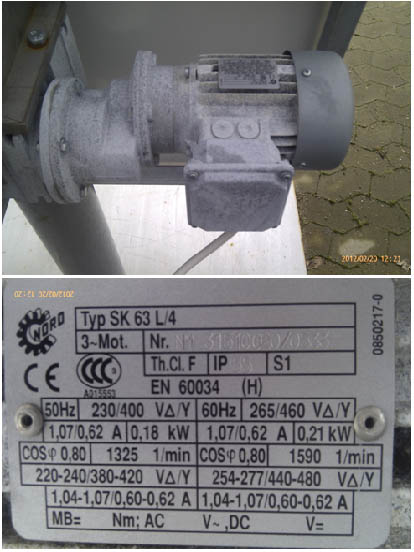
\includegraphics[scale=0.75]{images/oldmotor.jpg}
  \end{center}
  \caption{The Old Motor}
\end{wrapfigure}

% Bottom of the page
\end{document}